\chapter{Linux on z}
\label{cha:Linux_on_z}

\textit{Linux on z} oder abgekuerzt \textit{LoZ} ist ein Sammelbegriff fuer Linux Distributionen welche auf einem IBM Mainframe laufen. Dies sind vorallem IBMs z Systems und der IBM LinuxONE Server.\cite{LinuxOnZWiki}

Im Jahr 1999 hat IBM mehrere Patches, welche hauptsaehlich aus \textit{object code only} (OCO) Modulen bestanden, fuer den damals aktuellen Linux Kernel 2.2.13 veroeffentlicht.
Ungefaehr ein Jahr spaeter hat IBM diese OCO Module durch Open Source Module im Kernel ersetzt und Linux on z formal als IBM Produkt vorgestellt.\cite{LinuxOnZWikiHistory}

\section{Integrated Facility for Linux (IFL)}

In einer IBM Mainframe Umgebung werden dem Kunden pro Taktzyklus eines General Purpose Processors (CP) Nutzungsgebuehren verrechnet.
Um diese Kosten zu senken hat IBM drei spezielle Arten von Prozessoren entwickelt bei denen geringere Nutzungsgebuehren anfallen:
\begin{description}
    \item[zAAP]{Steht fuer \textit{z Systems Application Assist Processor} und wird genutzt um Java Workload auszufuehren\cite{IBMzAAP}}
    \item[zIIP]{Steht fuer \textit{z Systems Integrated Information Processor} und wird vorallem genutzt, um DB2 Workload auszufuehren\cite{IBMzIIP}}
    \item[IFL]{Steht fuer \textit{Integrated Facility for Linux} und wird genutzt, um Linux Workload auszufuehren\cite{IBMIFL}}
\end{description}
Der IFL ist hardware-technisch nichts anderes als ein Standard CP mit dem Unterschied, dass der Microcode die CP auf Linux und z/VM Instruktionen beschraenkt.

\section{Hauptmerkmale von Linux on z}

Das Ziel von Linux on z ist es die Vorteile eines IBM Mainframes mit einem Linux Betriebssystems zu nutzen, sodass Linux seine Charakteristiken behalten kann.

Das “Look \& Feel” von Linux on z soll dem entsprechen, was sich ein erfahrener Linux User gewohnt ist. Dazu gehoeren unter anderem:

\begin{itemize}
    \item{Linux als ASCII Environment}
    \item{Konform zum Linux Standard Base (LSB) und zum Filesystem Hierarchy Standard (FHS) Kompatibel mit POSIX}
    \item{Kein eigener Linux Kernel Fork fuer Linux on z -- Alles soll in Mainline Linux verfuegbar sein}
\end{itemize}

Die folgende Grafik zeigt, welche Linux- und GNU toolchain-Komponenten kleine Codeaenderungen zu Nutze machen muessen um auf einem Mainframe zu laufen:

\begin{figure}[h!]
\centering
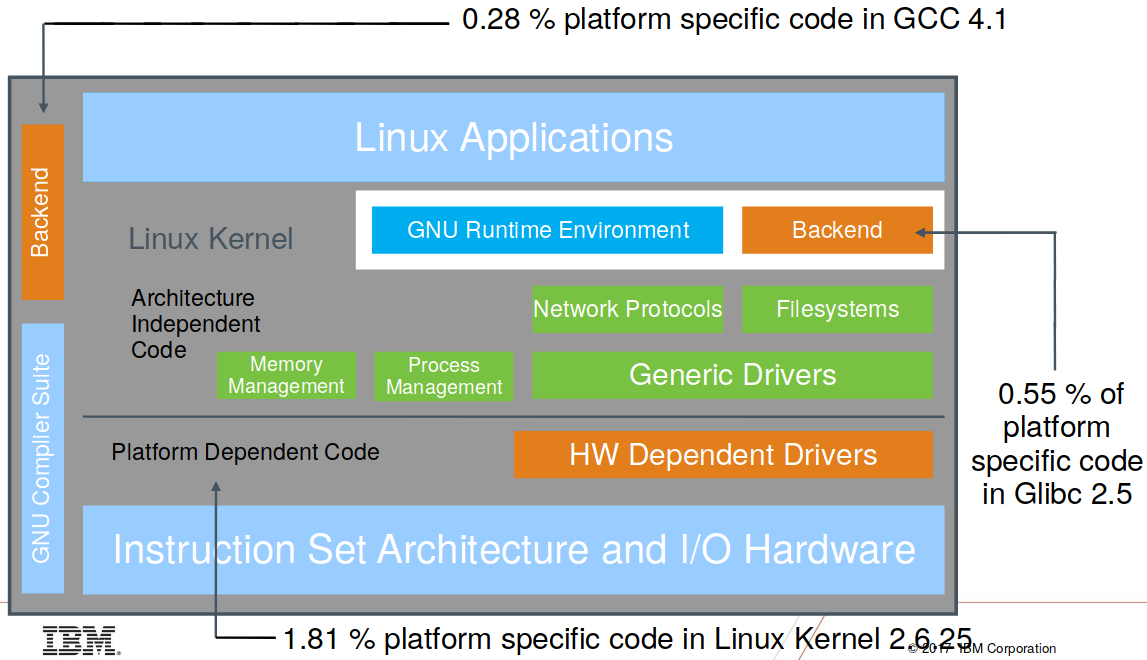
\includegraphics[width=.95\textwidth]{linux-on-z-kernel-struktur.png}
\caption{Linux on z Kernel\cite{LinuxOnZKernel}.}
\label{fig:LinuxOnZKernel}
\end{figure}

Wie man von der Grafik entnehmen kann, war dies der Stand des bereits fast 10 Jahre alten Linux Kernels 2.6.25.

Heute sind noch immer kleine Mainframe Plattform spezifische Aenderungen vorhanden, jedoch im Bereich von nur einem 1\%\cite{LinuxOnZSpecCode} -- Und diese sind im Mainline Kernel bereits enthalten, was einen Fork nicht noetig macht.

\section{IBM Mainframe Eigenschaften fuer Linux}

Wie schon im letzten Kapitel angeschnitten, ist ein grosses Ziel von Linux on z die Vorteile eines IBM Mainframes fuer Linux nutzen zu koennen.

IBM macht mit Linux on z folgende Angebote fuer Linux nutzbar:

\begin{figure}[h!]
\centering
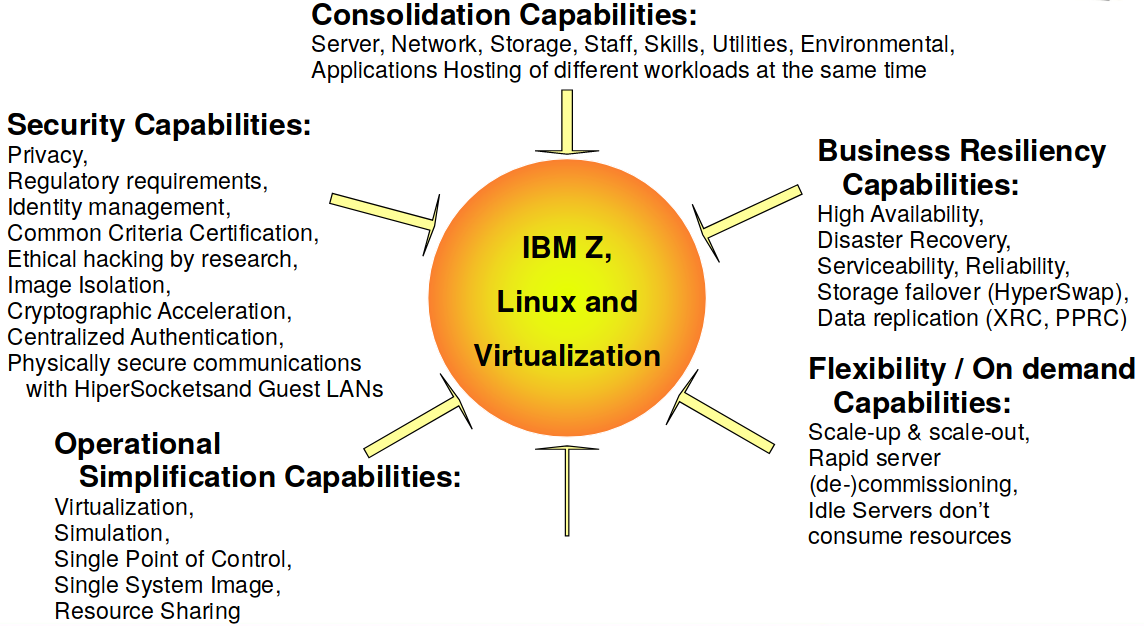
\includegraphics[width=.80\textwidth]{linux-on-z-mainframe-vorteile.png}
\caption{Linux on z Mainframe Vorteile\cite{LinuxOnZMainframeVorteile}.}
\label{fig:LinuxOnZMainframeVorteile}
\end{figure}

\begin{description}
    \item[Konsolidierung]{Das vereinen von Serverfarmen inklusive Netwerk und Storage Komponenten in einem einzigen Mainframe.}
    \item[Sicherheit]{Die IBM System z Plattform hat die EAL 5+\footnote{Siehe \url{https://en.wikipedia.org/wiki/Evaluation_Assurance_Level}} Sicherheits Zertifizierung erreicht. Auch z/VM, unter welcher Linux virtualisiert werden kann, kommt mit EAL 4+.}
    \item[Business Resiliency]{Die N+1 Ausfallsicherheit eines Mainframes kommt auch LoZ zu gute.}
    \item[Flexibilitaet]{Das Scale-up \& Scale-out Prinzip von den Mainframes gilt auch fuer LoZ.}
\end{description}

\section{Ziel Plattformen von LoZ}

Linux on z kann auf zwei verschiedene Arten auf einem Mainframe laufen: in LPARs oder als virtuelle Maschine unter z/VM. Aeltere Linux on z, welche noch fuer S/390 31-Bit Hardware entwickelt wurden, konnten auch direkt ohne Virtualisierung auf einem Mainframe laufen.
Fuer aktuelle 64-Bit S/390x Linux on z ist dies nicht mehr moeglich.

\subsection{Linux on z in LPARs}

Linux on z kann auf einem oder mehreren Logical Partitions (LPARs) installiert und laufen gelassen werden. Aktuelle z14 Mainframes unterstuetzen bis zu 85 LPARs -- es koennten also theoretisch 85 Linux on z Instanzen auf einem einzigen Mainframe laufen, ohne dass VMs zum Einsatz kommen.
Es ist auch moeglich nur auf einem Teil der LPARs Linux zu installieren und auf anderen LPARs ein anderes Mainframe Betriebssystem, wie z.B. z/OS:

\begin{figure}[h!]
\centering
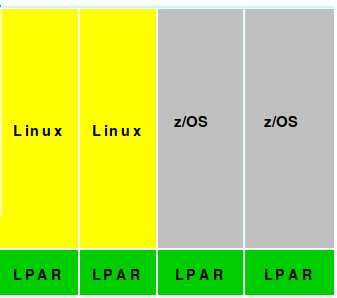
\includegraphics[width=.75\textwidth]{linux-on-z-linux-on-lpar.png}
\caption{Linux on z in LPARs\cite{LinuxOnZOnLPAR}.}
\label{fig:LinuxOnZOnLPAR}
\end{figure}

\subsection{Linux on z in z/VM}

Die zweite Moeglichkeit wie Linux on z auf einem Mainframe laufen gelassen werden kann, ist mit Hilfe einer Virtualisierung durch z/VM. Dabei wird Linux on z in einer full-virtualized Virtuelle Maschinen betrieben. z/VM wird in dieser Varianten selbst auch in eine LPAR installiert:

\begin{figure}[h!]
\centering
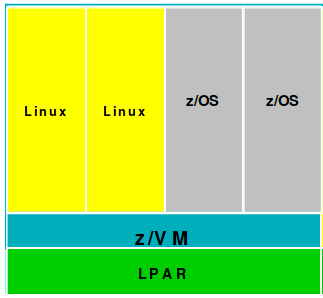
\includegraphics[width=.75\textwidth]{linux-on-z-linux-on-zvm.png}
\caption{Linux on z unter z/VM\cite{LinuxOnZOnZVM}.}
\label{fig:LinuxOnZOnZVM}
\end{figure}

\subsection{Linux on z: LPAR oder z/VM?}

Bei der Entscheidung ob Linux on z in einer LPAR oder unter z/VM installiert werden soll, spielen viele Faktoren eine Rolle:

\begin{description}
    \item[Anzahl der gewuenschten Linux Instanzen]{LPARs sind auf 86 Stück gegrenzt, wobei jede LPAR ihren eigenen physikalischen Arbeitsspeicher braucht. Weiter ist es einfacher grössere Mengen von Instanzen mit z/VM zu verwalten als in LPARs.}
    \item[Kommunikation zwischen verschiedenen Instanzen]{Zwischen z/VM Instanzen gibt es virtuelle Verbindungen und zwischen LPARs wird die Kommunikation mit HiperSockets gemacht. Je nach dem kann das eine oder andere Geschwindigkeitsvorteile mit sich bringen.}
    \item[Muessen andere Server auf dem gleichen Mainframe laufen]{Wenn andere Server ausser Linux Server auf dem selben Mainframe laufen muessen, koennen je nach dem LPARs oder z/VMs Vorteile bringen}
\end{description}

Grundsaetzlich kann man sagen, dass eine Linux Virtualisierung mit z/VM mehr Flexibilitaet und Skalierbarkeit verspricht.\cite{IBMzVMLPAR}

Es ist auch moeglich LPARs und z/VM Linux on z Instanzen auf einem Mainframe zu mischen:

\begin{figure}[ht!]
\centering
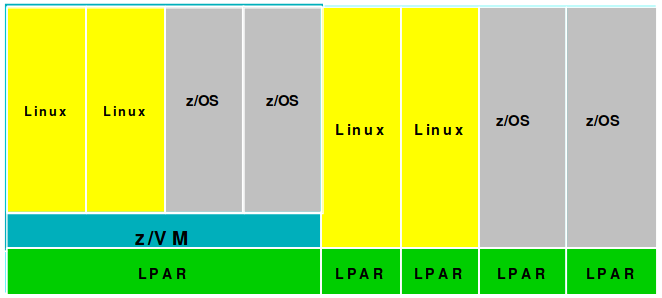
\includegraphics[width=.75\textwidth]{linux-on-z-linux-on-lpar-zvm.png}
\caption{Linux on z in LPARs und unter z/VM\cite{LinuxOnZOnLPARZVM}.}
\label{fig:LinuxOnZOnLPARZVM}
\end{figure}
